\section{ARMA Models}
% 2022-11-15

\begin{definition}{Stationary process (weakly stationary)}{}
    
    Gaussian process $\{X_t\},\,t=1,/ldots,n$
    \begin{align*}
        X &= (X_t) \sim \text{Multivariate Gaussian/Normal distribution} \\
        E(X) &= \mu = \left( \mu_1, \ldots, \mu_n \right)' \\
    \end{align*}

    The Covariance matrix $(n \times n)$ is given by:
    \begin{equation*}
        V(X) = \Gamma = \left\{ \gamma(t_i,t_j) \mid t,j = 1,\ldots,n\right\}
    \end{equation*}

    And the multivariate Normal density function can be written as:
    \begin{equation*}
        f(x) = (2\pi)^{-n/2} |\Gamma|^{-1/2} \text{exp}\left\{ -\frac{1}{2}(x-\mu)' \Gamma^{-1} (x-\mu) \right\}
    \end{equation*}
    where $|\Gamma|$ is the determinant of $\Gamma$.
\end{definition}

\begin{definition}{General Stochastic model for a time series}{}
    \begin{equation*}
        X_t = G\left(
            X_{t-1},\,X_{t-2},\,\ldots,\,Z_{t-1},\,Z_{t-2},\,\ldots
        \right) + Z_t, \quad Z_t \sim \mathcal{WN}(\sigma^2)
    \end{equation*}
    where $G$ is a deterministic function and $Z_t$ is a white noise process.
\end{definition}

\begin{definition}{Linear Stochastic model for a time series}{}
    \begin{align*}
        X_t = \sum_{i=1}^p \phi_i X_{t-i} + \sum_{j=1}^q \theta_j Z_{t-j} + Z_t, &&Z_t \sim \mathcal{WN}(\sigma^2) \\
        && \phi_1,\,\ldots,\,\phi_p,\,\theta_1,\,\ldots,\,\theta_q \in \mathbb{R}
    \end{align*}
    where $Z_t$ is a white noise process.

    The variable at time $t$ is a \iemph{linear combination} of past observations
    and disturbances plus a new disturbance independent from the past.
\end{definition}

\begin{definition}{$p$-th order Auto-Regressive Model (AR($p$))}{}
    \begin{align*}
        X_t &= \sum_{i=1}^p \phi_i X_{t-i} + Z_t \\
        Z_t &= \left(
            1 - \sum_{i=1}^p \phi_i B^i
            \right) X_t
    \end{align*}
    where $B$ is the backward shift operator.

    \tcblower

    An AR($p$) model is a regression model with lagged values of the dependent
    variable in the independent variable positions, hence the name Auto-Regressive.
\end{definition}






\begin{definition}{Stochastic processes (ARMA)}{}
	\begin{equation*}
		\text{ARMA}(p,q) \equiv \text{AR}(p) + \text{MA}(q)
	\end{equation*}
	\begin{equation*}
		X_t = \underbrace{
			\sum_{i=1}^p \phi_i X_{t-i}
		}_{\text{AR}(p)}
		+ \underbrace{
			\sum_{i=1}^q \theta_i Z_{t-i}
		}_{\text{MA}(q)}
		+ \underbrace{
			Z_t
			\vphantom{\sum_{i=1}^q}
		}_{ \substack{\text{Random} \\ \text{component}} }
		\quad \text{where} \; Z_t \sim \mathcal{N}(0,\,\sigma^2)
	\end{equation*}
	\begin{equation*}
		\text{ARMA}(p,q) \rightarrow \Phi_p(B) X_t = \Theta_q(B) Z_t
	\end{equation*}
\end{definition}


% TODO: idk
\begin{alignat*}{3}
	AR & (1) & \quad \rho(h) & = \phi^h                                       & \quad X_t   & = \phi X_{t-1} + Z_t \\
	AR & (p) & \quad \rho(h) & = \phi_1 \rho(h-1) + \cdots + \phi_p \rho(h-p) & \quad h > p
\end{alignat*}

\begin{alignat*}{3}
	MA & (1) & \quad \rho(h) & = \begin{cases}
		                             0                       & h > 1            \\
		                             \frac{\phi}{1-\theta^2} & \text{otherwise}
	                             \end{cases}                 \\
	MA & (q) & \quad \rho(h) & = \phi_1 \rho(h-1) + \cdots + \phi_p \rho(h-p) & \quad h > p
\end{alignat*}

We have a decreasing pattern (damped oscillations) for $h > p$ with
an infinite number of oscillations.

The last lag different from zero on the ACF of MA gives us the $q$.

PACF and ACF are complementary on AR and MA processes.

\begin{equation*}
	V(\hat \rho (h))  \approxeq \frac{1}{T}
\end{equation*}
\begin{equation*}
	s(\hat \rho (h))  = \sqrt{V(\hat \rho (h))} \approxeq \frac{1}{\sqrt{T}}
\end{equation*}

\begin{align*}
	H_0 & : \hat \rho (h) = 0    \\
	H_1 & : \hat \rho (h) \neq 0
\end{align*}

If the estimation lies within the confidence interval
$\hat \rho (h) \in \left[-\frac{1.96}{\sqrt{T}}, \frac{1.96}{\sqrt{T}}\right]$,
we cannot reject the null hypothesis $H_0$.

\begin{note}
	We cannot always rely on this confidence interval.

	Remember that what we care about is which is the last one which is not
	equal to zero.

	We should only apply it for the initial lags, not for lags greater
	than 0 that are well in the past.
\end{note}

\begin{marker}
	Common mistake: if we identify in a plot a AR or MA, we don't have an
	ARMA (AR(p) implies MA(infinity) and vice versa).

	We cannot find the p, and q for ARMA(p, q) from the ACF and PACF.
\end{marker}

\begin{figure}[H]
	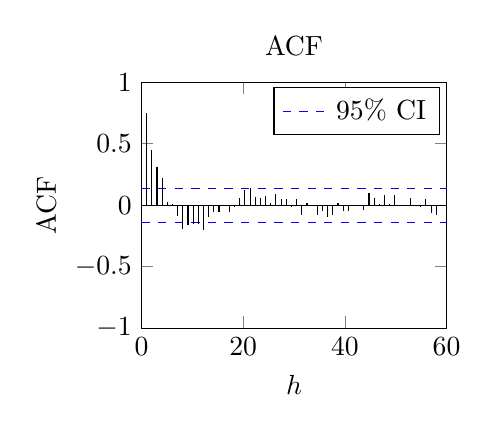
\begin{tikzpicture}
		\begin{axis}[
				ymin=-1, ymax=1,
				enlargelimits=false,
				width=0.45\textwidth,
				title=ACF,
				xlabel=$h$,
				ylabel=ACF,
			]
			% set pgf math constant
			\pgfmathsetmacro{\T}{200}
			\pgfmathsetmacro{\mx}{60}
			\pgfmathsetmacro{\ci}{1.96/sqrt(\T)}
			\addplot[blue, dashed, mark=none, samples=2, domain=0:\mx] {\ci};
			\addlegendentry{95\% CI};
			\addplot[blue, dashed, mark=none, samples=2, domain=0:\mx] {-\ci};
			\addplot[black, mark=none, samples=2, domain=0:\mx] {0};
			\addplot[ycomb,samples=\mx, domain=0:\mx, mark=none] {2.5*cos(\x*15)/(\x+2.5) + rand*\ci/2};
			% \addplot[ycomb, domain=0:\mx, mark=none] {cos(\x*15)};
		\end{axis}
	\end{tikzpicture}
	\hfill
	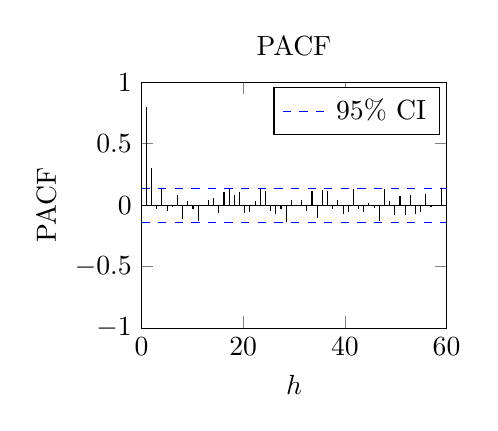
\begin{tikzpicture}
		\begin{axis}[
				ymin=-1, ymax=1,
				enlargelimits=false,
				width=0.45\textwidth,
				title=PACF,
				xlabel=$h$,
				ylabel=PACF,
			]
			% set pgf math constant
			\pgfmathsetmacro{\T}{200}
			\pgfmathsetmacro{\mx}{60}
			\pgfmathsetmacro{\ci}{1.96/sqrt(\T)}
			\addplot[blue, dashed, mark=none, samples=2, domain=0:\mx] {\ci};
			\addlegendentry{95\% CI};
			\addplot[blue, dashed, mark=none, samples=2, domain=0:\mx] {-\ci};
			\addplot[black, mark=none, samples=2, domain=0:\mx] {0};
			\addplot[ycomb,samples=\mx-3, domain=3:\mx, mark=none] {rand*\ci};
			\addplot[ycomb] coordinates {
					(0, 0)
					(1, 0.8)
					(2, 0.3)
				};
		\end{axis}
	\end{tikzpicture}
	\caption{ACF and PACF}
\end{figure}

\subsection{ARIMA}

ARIMA(p,d,q)

AR = auto correlation
I =
MA = Moving average

significant test

% t  = phi/s

% H_0 = phi_i = 0

% if t is > 2 then H_0 rejected

which means that phi must be kept in the value.

(is the coeficient is more than two times the absolute value)
